\documentclass[11pt,a4paper]{ctexart}
\usepackage[margin=1.75cm]{geometry}
\usepackage{amsmath,amssymb,bm}
\usepackage{booktabs,graphicx,xcolor,hyperref,array,float,tabularx}
\hypersetup{colorlinks=true,linkcolor=blue,urlcolor=blue,citecolor=blue}
\setlength{\parindent}{2em}
\setlength{\parskip}{0.22em}
\newcommand{\norm}[1]{\left\lVert #1\right\rVert}
\newcommand{\med}{\operatorname{median}}
\title{IMU--UWB InEKF：Task06逐锚测距模型与鲁棒拒绝}
\author{LOSO离线标定、Huber降权、三维与XY双口径验证}
\date{2026年8月3日}

\begin{document}
\pagestyle{plain}
\maketitle

\begin{abstract}
原Task06对八个锚点统一使用距离偏差$-0.18$ m、标准差$0.20$ m及
$\epsilon>25$（约5$\sigma$）硬拒绝。本轮只改测量模型与异常处理：对每条
待测日志，从其余11条日志冻结逐锚中位偏差和$1.4826\,\mathrm{MAD}$尺度；
初始化256次更新后，对2--3.5$\sigma$创新连续Huber降权，超过3.5$\sigma$
硬拒绝。待测日志OptiTrack只用于事后评分，不向滤波器注入位置或高度。

12条TU Delft TWR日志上，nominal普通TWR--InEKF、direct TWR与lifted
TWR的三维RMSE中位数分别由$0.346/0.387/0.404$ m降到
$0.328/0.333/0.358$ m；XY中位数分别降到$0.173/0.174/0.173$ m。
9 m初差下三种方法均12/12收敛。组件消融显示逐锚模型贡献主要精度收益，
鲁棒门控负责避免窄逐锚噪声导致的大初差门控锁死。改进后z轴仍占约
$76\%$--$80\%$平方误差，剩余瓶颈仍是垂直几何，而非继续收紧门限即可消除。
\end{abstract}

\section{范围与公平协议}

状态方程、IMU初始化、有效加速度过程噪声、锚点坐标、零延时数据加载、
初始偏移及评分窗口均保持原Task06不变。真实实验为12条日志、零初差与
$[6,-6,3]^\top$ m（范数9 m）两种初值、direct TWR、普通TWR--InEKF和
lifted TWR三种结构。原尾段流形消融与20次Theodosis单锚点Monte Carlo
重新执行；新增所有位置/速度的XY指标。

对于第$j$条待测日志，只允许用$\mathcal D_{-j}$中其余11条日志标定。
这属于带监督的离线传感器标定；它仍需要独立标定数据，但不同于连续运行时
读取当前评分真值的oracle辅助。待测日志真值不参与偏差、尺度、门限或状态更新。

\section{相对原Task06的数学改进}

\subsection{全局标量改为逐锚冻结参数}

原Task06固定
\begin{equation}
b_i\equiv-0.18\ {\rm m},\qquad \sigma_i\equiv0.20\ {\rm m}.
\label{eq:old-model}
\end{equation}
对训练日志中锚点$i$的异步事件，本轮定义
\begin{equation}
e_{k,i}=\widetilde\rho_{k,i}-\norm{p_k^{\rm gt}-a_i},
\end{equation}
并在每个LOSO折冻结
\begin{align}
\widehat b_i
 &=\med_{k\in\mathcal D_{-j}}e_{k,i},\\
\widehat\sigma_i
 &=\operatorname{clip}\!\left(
 1.4826\med_{k\in\mathcal D_{-j}}
 |e_{k,i}-\widehat b_i|,0.08,0.35\right)\ {\rm m}.
\label{eq:loso-model}
\end{align}
测试时只计算
\begin{equation}
\rho_{k,i}=\widetilde\rho_{k,i}-\widehat b_i.
\end{equation}
direct与普通InEKF取$R_i=\widehat\sigma_i^2$。原lifted半平方观测保持为
\begin{align}
y_{k,i}&=\frac12(\rho_{k,i}^2-\widehat\sigma_i^2),\\
R^{\rm sq}_{k,i}
 &=\rho_{k,i}^2\widehat\sigma_i^2+\frac12\widehat\sigma_i^4.
\label{eq:squared-noise}
\end{align}
因此本轮没有改变Task06的提升状态$q,s,h,p,v$或常观测行，只把错误的
同质测距假设替换为逐锚模型。

\begin{figure}[H]
 \centering
 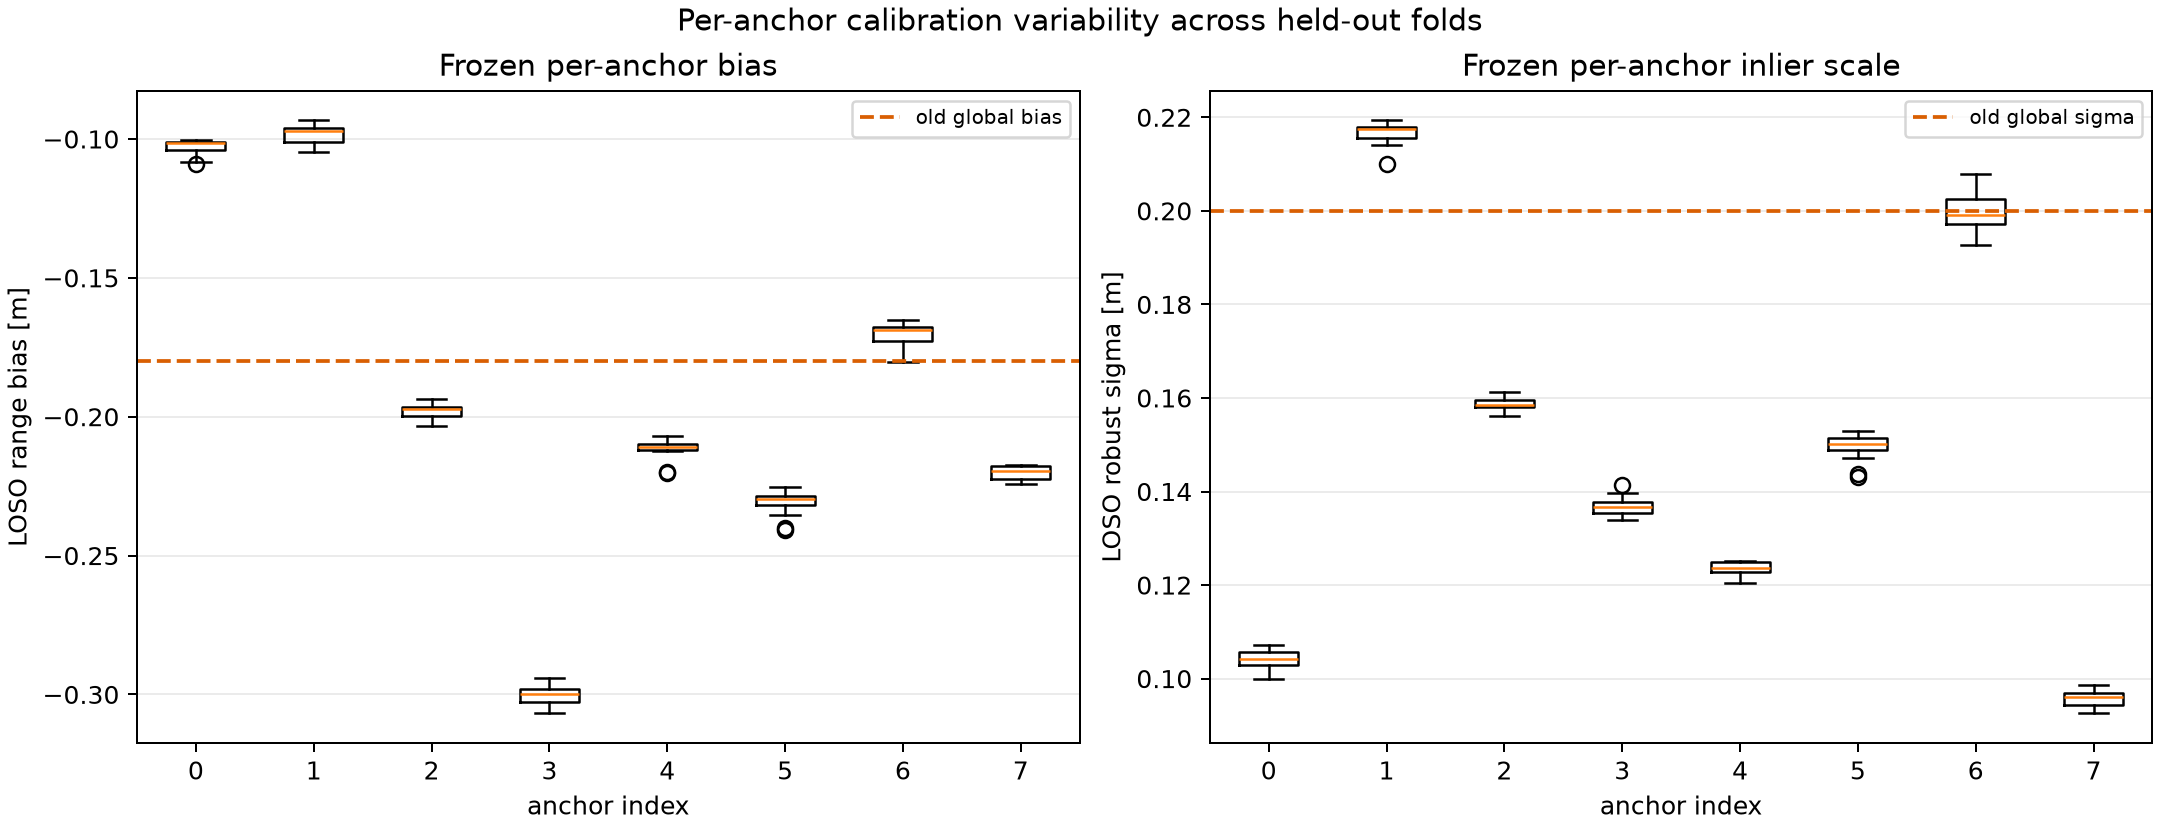
\includegraphics[width=\textwidth]{../imu-uwb-inekf-state-augment/results/task06_per_anchor_robust/improved_comparison/per_anchor_calibration.png}
 \caption{12个LOSO折中的逐锚偏差与稳健尺度。旧全局参数以虚线表示。}
 \label{fig:anchor-calibration}
\end{figure}

\subsection{旧五倍标准差硬门限改为软硬结合}

原Task06只判断
\begin{equation}
\epsilon_k=\frac{r_k^2}{H_kP_k^-H_k^\top+R_{k,i}}>25
\quad\Longrightarrow\quad\text{拒绝}.
\label{eq:old-gate}
\end{equation}
该门限对统一$0.20$ m尺度过宽，但直接把逐锚尺度接入旧64次预热又会在
大初差下过早锁门。本轮完成256次初始化更新后执行
\begin{align}
\epsilon_k&>12.25 \quad\Longrightarrow\quad\text{硬拒绝},\\
w_k&=\min\!\left(1,\frac{2}{\sqrt{\epsilon_k}}\right),\\
R_{k,i}^{\rm eff}&=\frac{R_{k,i}}{w_k}.
\label{eq:robust-gate}
\end{align}
即2$\sigma$内正常更新，2--3.5$\sigma$连续降权，3.5$\sigma$外拒绝。
Kalman增益和Joseph协方差更新均使用$R^{\rm eff}$。

64次正式初跑暴露4条direct大初差锁死；专项压力测试中128次仍失败2条，
256次四条均恢复到$0.320$--$0.524$ m，512/1024次无实质额外收益，故固定256。

\section{真实全批：原始三维与新增XY}

\begin{table}[H]
\centering\small
\caption{原模型到完整改进的12日志RMSE中位数。}
\begin{tabular}{llrrrr}
\toprule
初值 & 方法 & 原3D & 改3D & 原XY & 改XY\\
 & & \multicolumn{4}{c}{单位：m}\\
\midrule
nominal & direct TWR & 0.387111 & 0.332875 & 0.191767 & 0.174492\\
nominal & 普通TWR--InEKF & 0.346125 & 0.328305 & 0.189343 & 0.172807\\
nominal & lifted TWR & 0.404446 & 0.357657 & 0.189612 & 0.173223\\
9 m & direct TWR & 0.438736 & 0.390191 & 0.201931 & 0.182378\\
9 m & 普通TWR--InEKF & 0.418764 & 0.363082 & 0.196351 & 0.181108\\
9 m & lifted TWR & 0.407519 & 0.369823 & 0.199138 & 0.178332\\
\bottomrule
\end{tabular}
\label{tab:main-result}
\end{table}

\begin{table}[H]
\centering\small
\caption{最后5 s位置RMSE中位数：三维与XY。}
\begin{tabular}{llrrrr}
\toprule
初值 & 方法 & 原3D & 改3D & 原XY & 改XY\\
\midrule
nominal & direct TWR & 0.192065 & 0.143970 & 0.106810 & 0.080545\\
nominal & 普通TWR--InEKF & 0.201253 & 0.152438 & 0.106794 & 0.084469\\
nominal & lifted TWR & 0.334650 & 0.234830 & 0.108144 & 0.079344\\
9 m & direct TWR & 0.192065 & 0.143970 & 0.106810 & 0.080545\\
9 m & 普通TWR--InEKF & 0.229953 & 0.152280 & 0.115900 & 0.084543\\
9 m & lifted TWR & 0.334650 & 0.234830 & 0.108144 & 0.079344\\
\bottomrule
\end{tabular}
\end{table}

\begin{figure}[htbp]
 \centering
 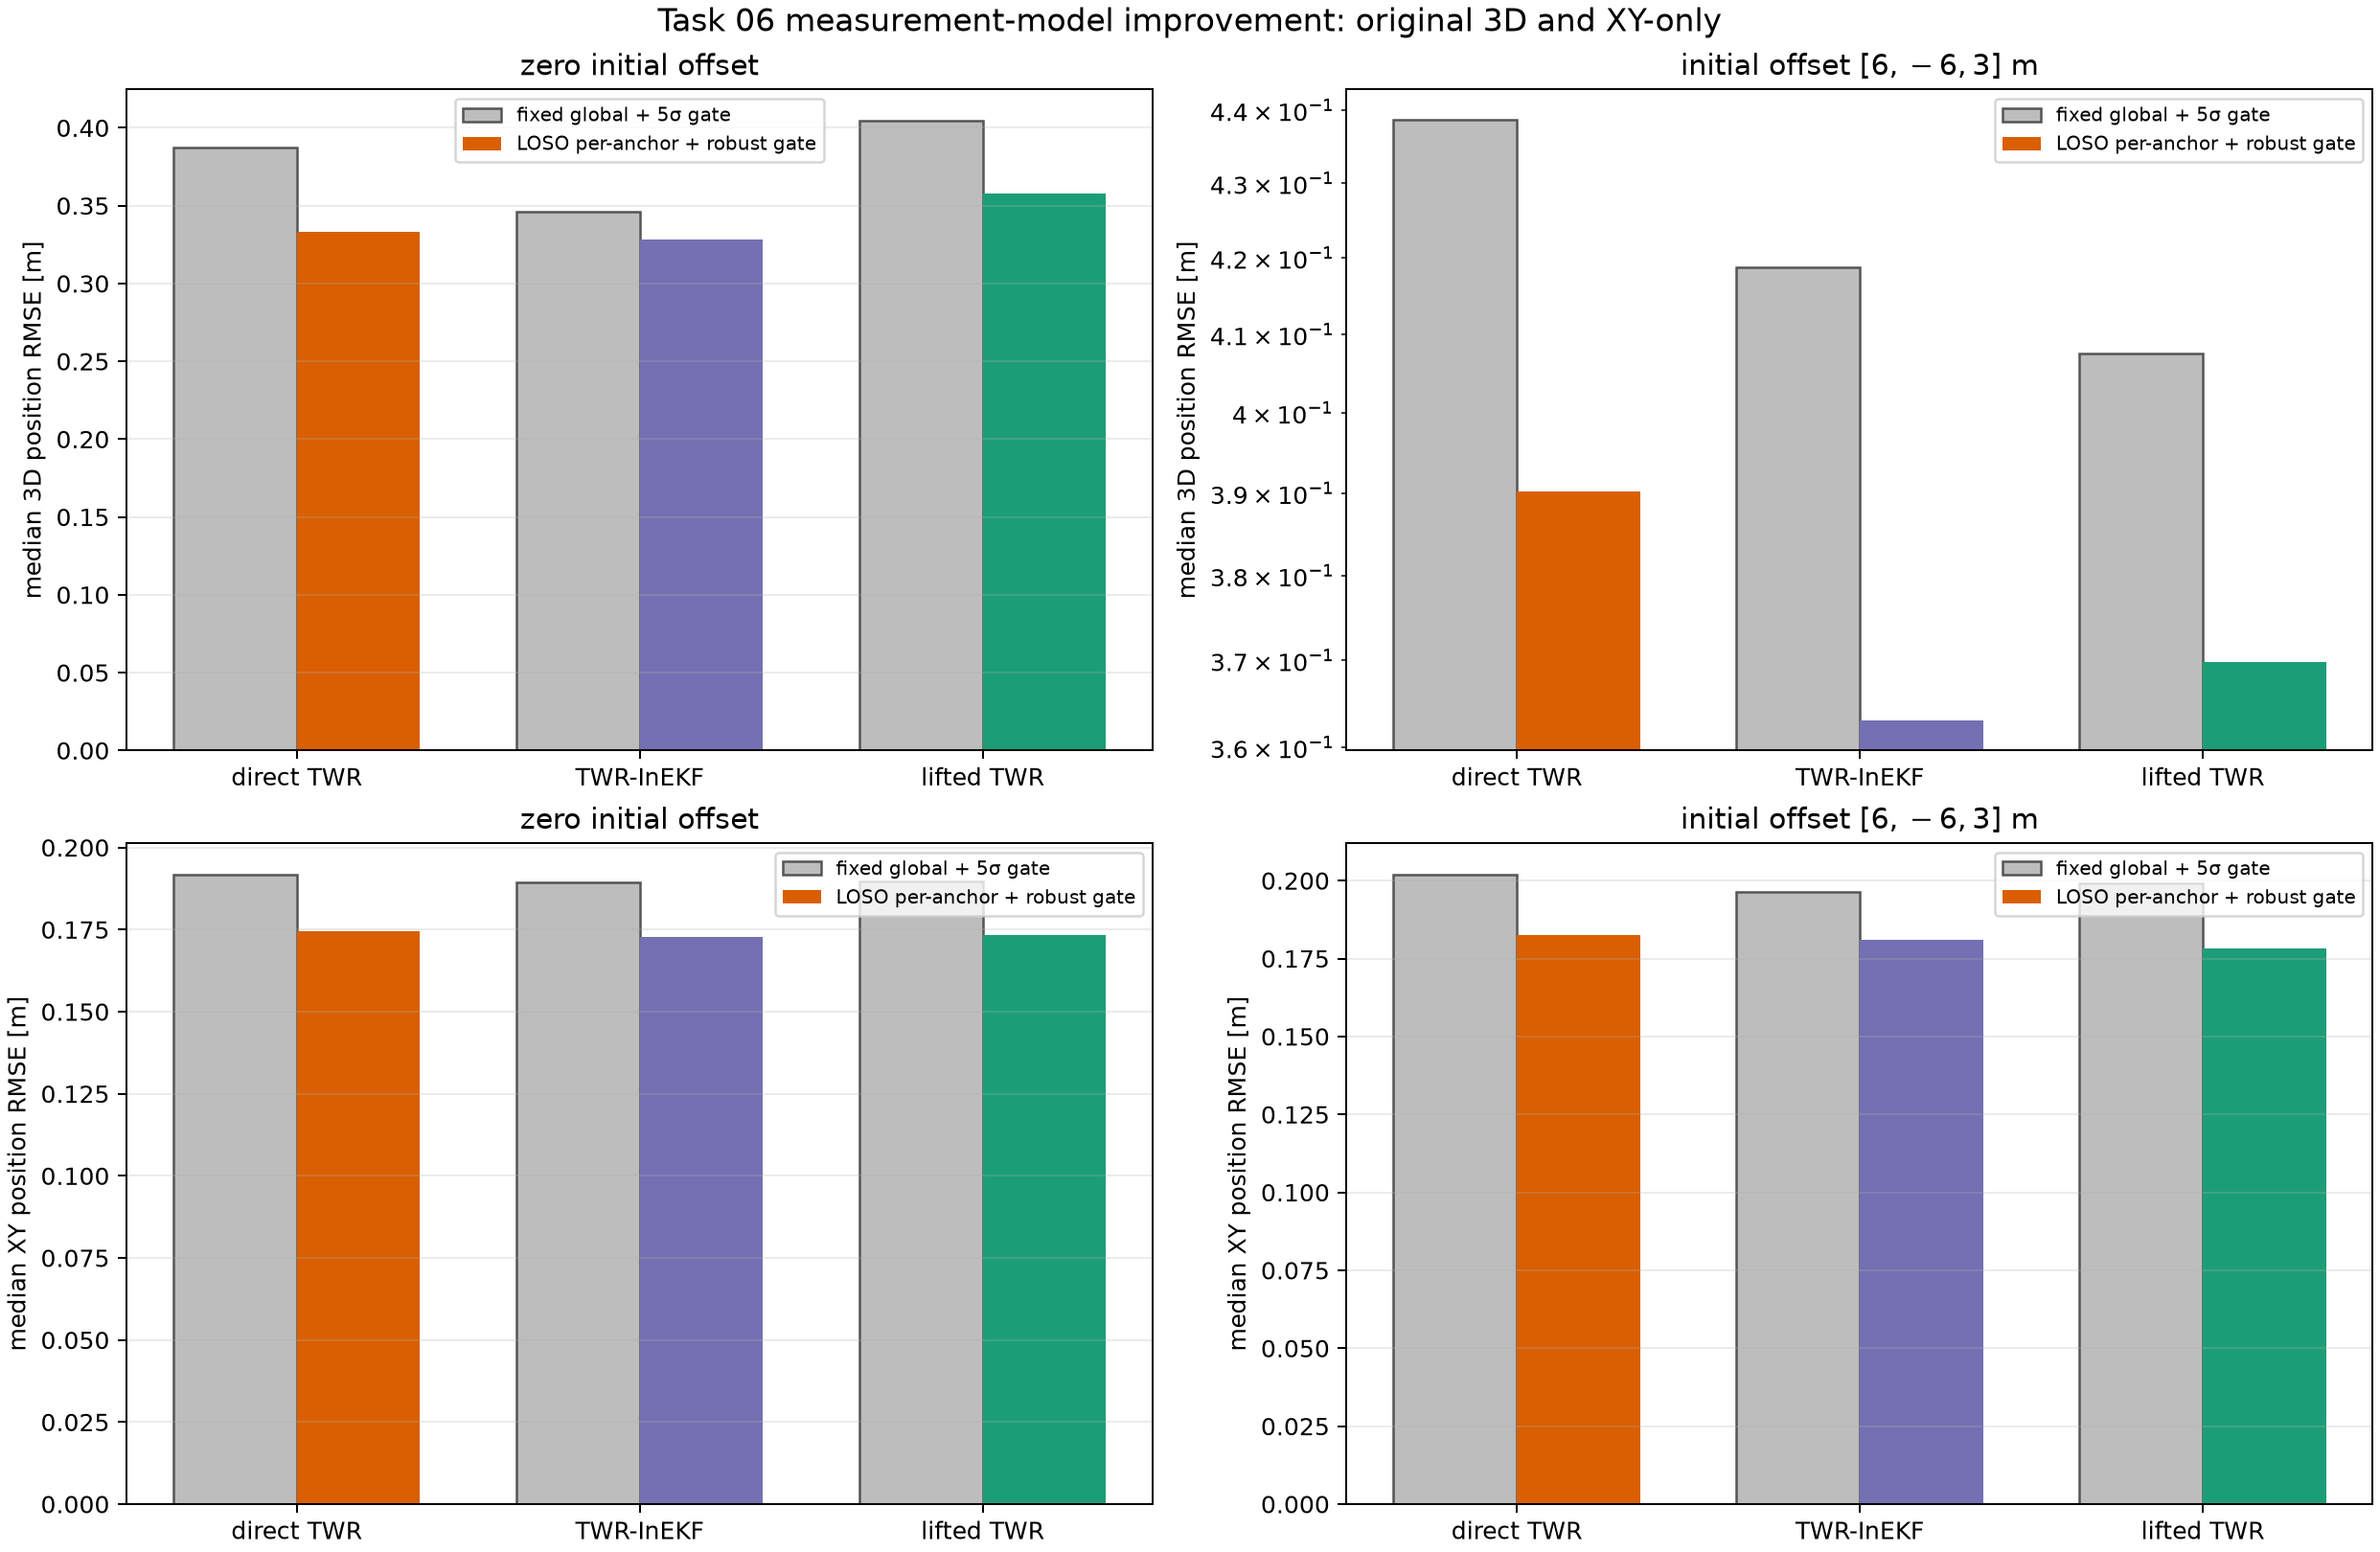
\includegraphics[width=\textwidth]{../imu-uwb-inekf-state-augment/results/task06_per_anchor_robust/improved_comparison/improvement_comparison.png}
 \caption{原全局模型与完整改进的3D/XY中位数。}
 \label{fig:main-comparison}
\end{figure}

nominal全程3D的逐日志改善数为direct $10/12$、普通InEKF $10/12$、
lifted $12/12$；全程XY三者均$12/12$改善。9 m时全程3D分别为
$11/12,10/12,12/12$。改进后三种方法均12/12进入0.5 m；普通InEKF仍有
一条到12.79 s才收敛，全程RMSE为1.554 m，未从统计中删除。

\section{组件消融：精度来自哪里}

\begin{table}[H]
\centering\small
\caption{nominal全程3D/XY中位数。}
\resizebox{\textwidth}{!}{%
\begin{tabular}{lrrr}
\toprule
配置 & direct 3D/XY & 普通InEKF 3D/XY & lifted 3D/XY\\
\midrule
全局参数+旧门控 & 0.387111/0.191767 & 0.346125/0.189343 & 0.404446/0.189612\\
逐锚参数+旧门控 & 0.336085/0.176344 & 0.331665/0.174385 & 0.362130/0.174696\\
全局参数+鲁棒门控 & 0.386530/0.191225 & 0.345634/0.188256 & 0.405712/0.188740\\
逐锚参数+鲁棒门控 & \textbf{0.332875/0.174492} & \textbf{0.328305/0.172807} & \textbf{0.357657/0.173223}\\
\bottomrule
\end{tabular}}
\end{table}

nominal精度主要来自逐锚模型；全局$0.20$ m下单独启用鲁棒门控几乎不改变
精度。大初差则不同：逐锚+旧门控的direct中位数虽为0.396 m，均值却因
锁死达到64.046 m；普通InEKF均值为6.723 m。全局+鲁棒门控将普通InEKF
均值从30.725 m降到0.848 m；两项同时启用进一步降到0.475 m。因此鲁棒
门控主要提供稳定吸引域，逐锚模型主要降低正常运行误差，二者有协同。

\begin{figure}[H]
 \centering
 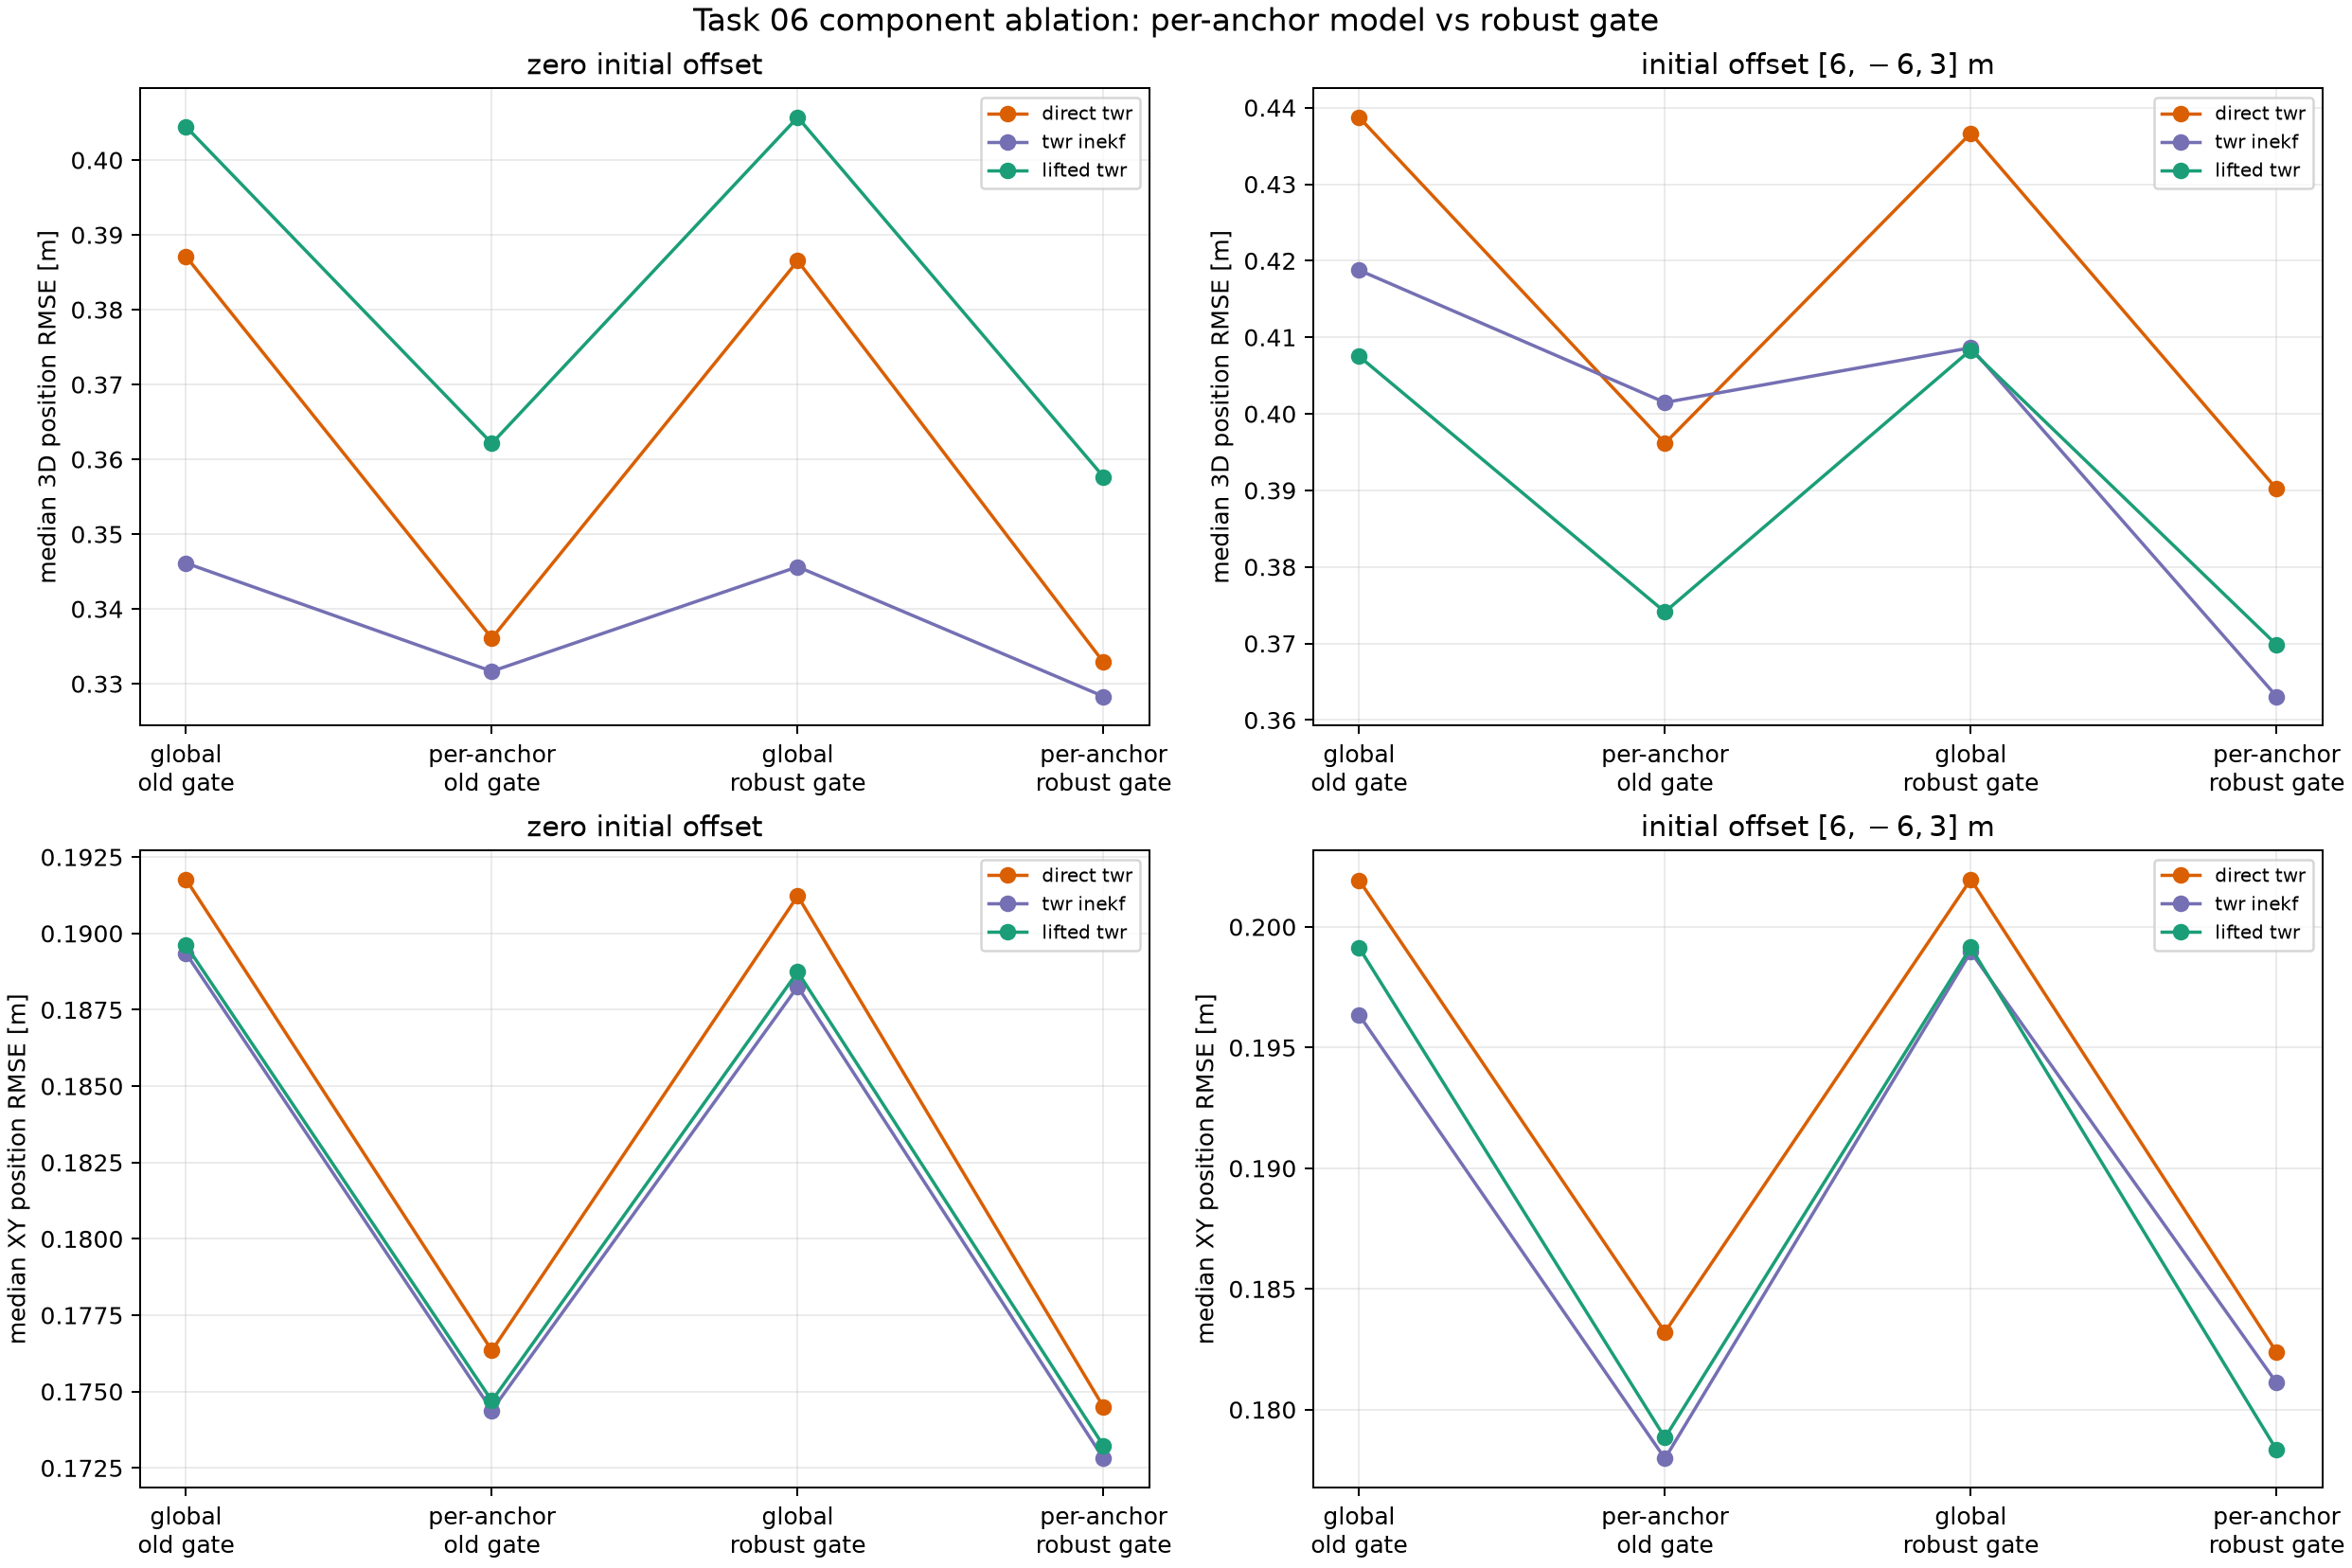
\includegraphics[width=\textwidth]{../imu-uwb-inekf-state-augment/results/task06_per_anchor_robust/component_ablation/component_ablation.png}
 \caption{逐锚模型与鲁棒门控的四配置组件消融。}
 \label{fig:component-ablation}
\end{figure}

\section{拒绝行为与剩余z轴瓶颈}

每个方法、每种初值均尝试149056次TWR更新。nominal下，direct/普通/lifted
旧硬拒绝为$66/72/69$次，新硬拒绝为$409/487/367$次，另有
$2083/2267/1783$次连续降权。硬拒绝率仍只有$0.25\%$--$0.33\%$，不是
大面积删量测。9 m原普通InEKF的19095次拒绝来自门控锁死，不代表异常识别
准确；改进后只有504次且12/12收敛。

\begin{figure}[H]
 \centering
 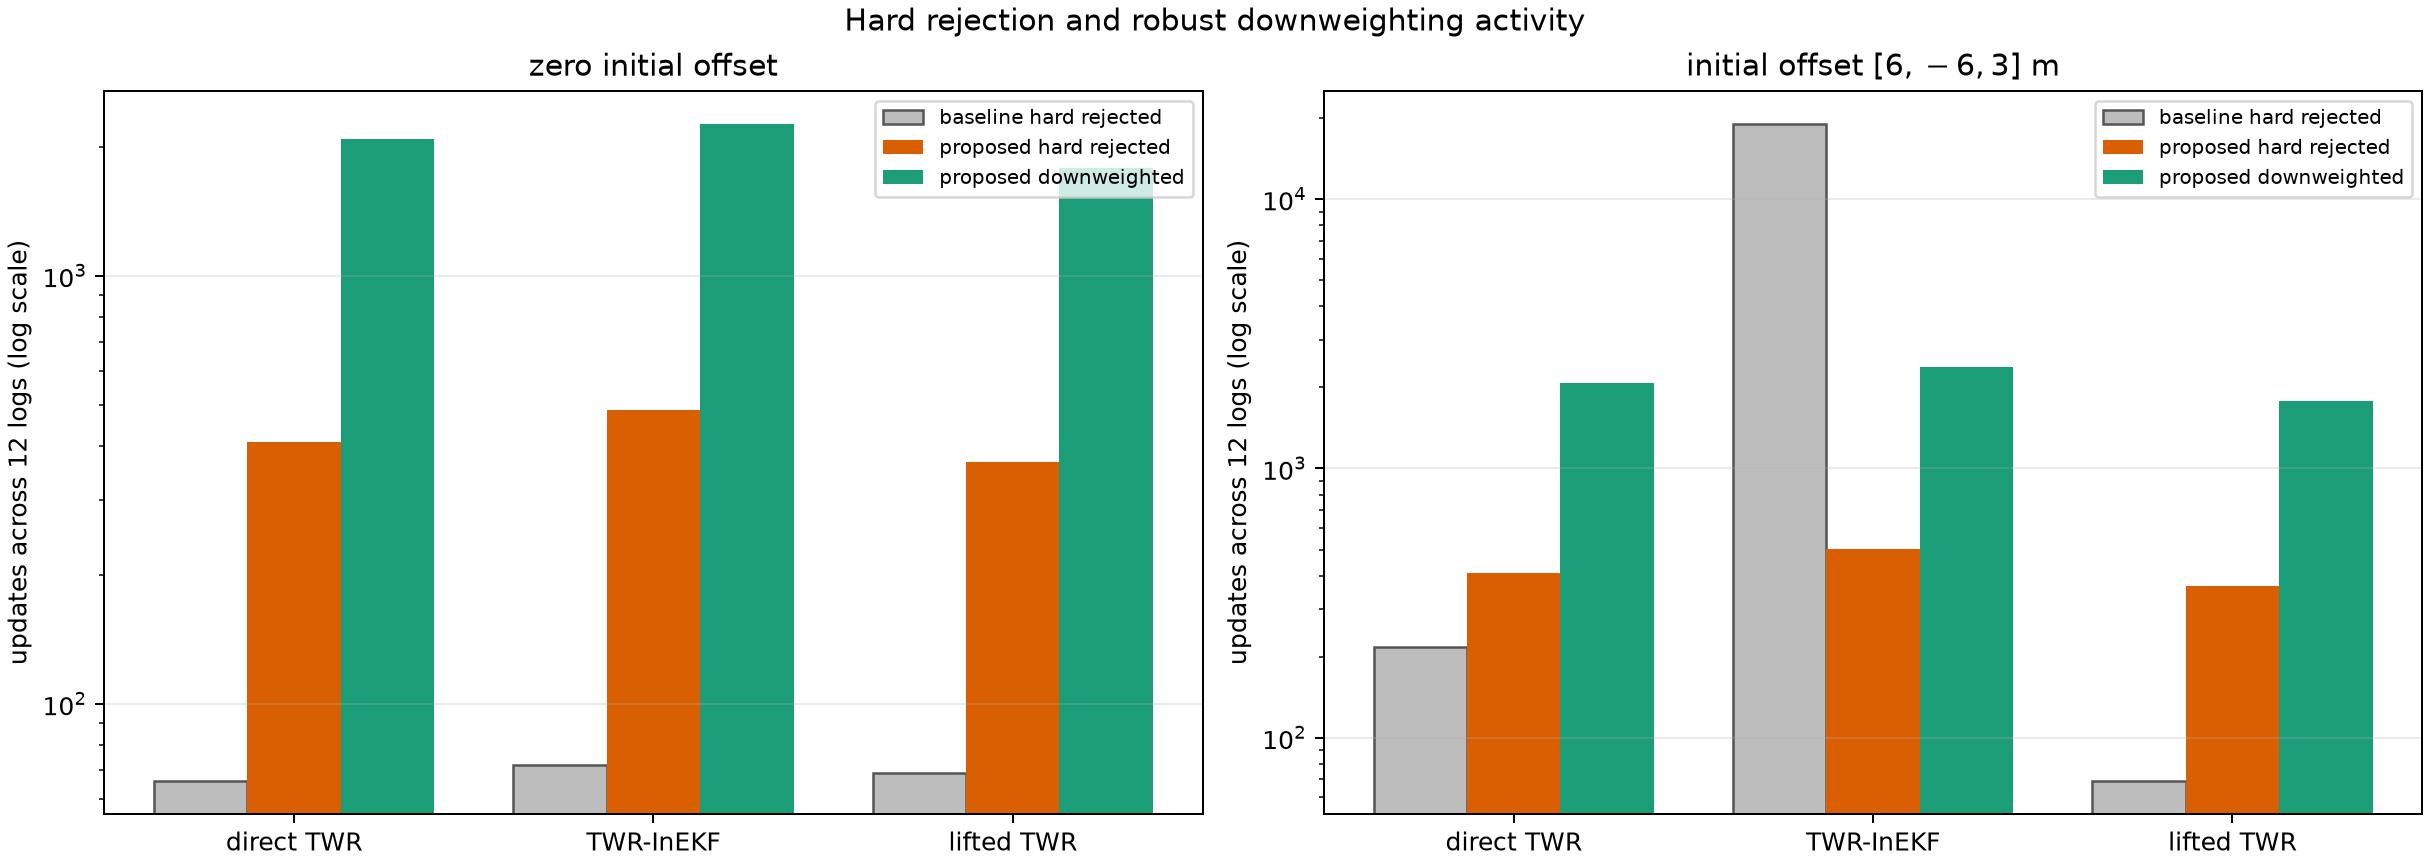
\includegraphics[width=\textwidth]{../imu-uwb-inekf-state-augment/results/task06_per_anchor_robust/improved_comparison/update_activity.png}
 \caption{硬拒绝与连续降权次数。纵轴为对数尺度。}
 \label{fig:update-activity}
\end{figure}

由同一轨迹的RMSE恒等式
\begin{equation}
\operatorname{RMSE}_z=
\sqrt{\operatorname{RMSE}_{3D}^2-\operatorname{RMSE}_{XY}^2}
\end{equation}
可得nominal改进direct/普通/lifted的z RMSE中位数为
$0.295/0.290/0.321$ m，z平方误差占比中位为$75.8\%/76.6\%/79.5\%$。
逐锚模型同时改善水平和垂直方向，但垂直误差仍主导，说明剩余差距主要由
锚点高度分布与纯测距垂直可观性决定。继续显著提升三维精度应优先考虑非真值
高度传感器、锚点垂直布设或专门的z方向约束，而不是继续压低硬门限。

\section{原Task06结论保留与验证}

原尾段机理消融的3D末5 s中位数仍为direct $0.192$ m、六维平方距离
$0.207$ m、lifted $0.335$ m、投影$0.207$ m；对应XY仅为
$0.107/0.105/0.108/0.105$ m。故lifted尾段惩罚仍主要来自$q,s,h$流形
漂移并集中于z方向，本轮没有偷换为投影算法。

20次Theodosis单锚点Monte Carlo保持原结论：lifted的3D和XY均20/20成功，
末5 s中位为$0.381/0.348$ m；direct和普通InEKF均0/20。逐锚真实标定未
移植到合成实验。

实现通过\texttt{compileall}及18/18项单元测试。256次修正版完整回放约
235 s，组件消融约180 s。原全批、改进、逐锚、门控活动、代表轨迹、尾段
3D/XY、synthetic与Monte Carlo图片均逐张目视检查；无NaN、断裂、错位或裁切。

需要保留三项边界：LOSO仍需外部标定日志；256次预热是本数据9 m压力测试
所得描述性常数；本轮按要求没有引入0.20 s时间修正或其他细微算法改动。

\end{document}
